\chapter{Using \headinglatin{\ksonline}}\label{ch:online}
\index{Online edition}

\ksonline{} brings the toolbox workspace to your browser without a local client installation. You edit structures, build workflows, and analyze results in the main window, while the server performs the calculations. The official Hanhai Quantum\regmark{} Online service is forthcoming, and private cluster deployments are supported. Sign in through the entry page provided by your deployment to open your allocated workspace.

Files and sessions are the main differences from the desktop application. Upload local inputs before using them, save projects in the server-side Files panel, and download them to obtain copies on your computer. Closing a page, returning to the entry page, and signing out also have different effects. This chapter connects these operations in a complete silicon-project exercise.

\section{Open your workspace}

\subsection{What you need}

Have the service address, a working account, and one of the small supplied structure files ready. Registration may require an invitation code; follow your deployment's registration instructions. Your browser must support WebGL to display atomic structures in 3D.

Use a reasonably large browser window. In a small window, both the central view and parameter editor become narrow, and long forms may require scrolling. On a laptop, collapse side panels you are not using to leave more room for the ribbon and active document.

Use one active browser tab per workspace. If the workspace is open in another tab, return to that tab or close the old connection before reconnecting.

\subsection{Register an account}

The service entry page initially displays the sign-in form. To create an account, switch to registration and complete the fields in order. Usernames must start with a letter and contain 3--32 lowercase letters, digits, or hyphens. Passwords must contain 12--128 characters and be entered again for confirmation.

Registration also requires a recovery question, recovery answer, and invitation code. Choose a question and answer you can remember without disclosing your password. Complete the form, register the account, and return to sign-in after registration succeeds.

\subsection{Sign in and wait for startup}

\begin{steps}
\item Enter your account details on the service entry page.
\item Choose the action to sign in and open the workspace.
\item Wait while the entry page reports workspace preparation. The first startup may take longer.
\item Enter the toolbox when the workspace is ready. If the entry page displays an action to open the workspace, select it.
\item Check that the ribbon is visible, that the \ui{Project Browser} and \ui{Files} panels can be opened on the left, and that the central document area responds.
\end{steps}

The portal may report states such as starting and ready. Keep the page open as the state changes; repeatedly clicking the startup action is unnecessary. If your organization has reached its concurrent-workspace limit, follow the portal's instructions and try again later. The deployment administrator determines whether capacity can be increased.

\section{Understand Online files}
\index{Server-side files}

\subsection{The project tree and file tree}

Use the left-side buttons to switch between the Project Browser and Files panel. They occupy the same area, with one shown at a time. Return to the Project Browser to work with structures, or switch to Files to inspect uploaded files.

The Project Browser organizes the contents of the current project: structures, workflows, calculation data, and figures. The \ui{Files} panel shows files and folders in server-side storage. A single \file{.ks} file can contain many project items, so the two trees show different things.

Think of a project as a notebook holding your structures and results, and the server-side folder as the shelf where notebooks are stored. Importing adds material to the notebook; saving writes the notebook to a \file{.ks} file. Uploading a CIF only places the source material on the shelf; it does not yet add it to the current project.

\begin{table}[htbp]
\centering
\caption{What common file operations do.}
\begin{tabularx}{\linewidth}{lX}
\toprule
Operation & Result \\
\midrule
Upload & Copies a local file into the current server-side directory.\\
Import & Reads a file and adds a structure, workflow, or other object to the project.\\
Save & Writes the current project to a server-side \file{.ks} file.\\
Download & Saves a copy of the selected server-side file on your computer.\\
Open project & Reads a \file{.ks} file as the current project.\\
\bottomrule
\end{tabularx}
\end{table}

\subsection{Everyday operations in Files}

The tree is sorted by name, with folders before files. Expand a folder to see its contents. The header arrow switches between ascending and descending order. Open the \ui{⋮} menu or right-click an item for file actions.

When a folder is selected, its path appears at the bottom of the panel. Selecting a file also shows its size. Upload, New folder, and the first project save use the current directory, so check that path before proceeding.

\ui{Refresh} rereads the directory and normally preserves expanded folders and the selection. If a new file is not visible after another operation, refresh and check that the correct folder is expanded. Organizing files by study or exercise is easier than repeatedly searching a long directory listing.

Figure~\ref{fig:online-workspace-silicon} shows this exercise after saving, with Files on the left. Use the Project Browser's side button to return to structures and workflows inside the project.

\section{Exercise: create a silicon project}

\subsection{Create an exercise directory}

Use the supplied \file{examples/silicon.cif}. The same file operations apply to another small structure. Start with a separate directory so that source structures, working projects, and downloaded copies are easy to distinguish.

\begin{steps}
\item In \ui{Files}, select the root or your chosen working directory.
\item Choose \ui{⋮ → New folder} and enter \file{Si-study}.
\item Check that the folder appears, then select and expand it.
\item Check the path at the bottom of the panel to confirm that \file{Si-study} is the current destination.
\end{steps}

\subsection{Upload the structure}
\index{Uploading files}

\begin{steps}
\item Choose \ui{Upload} in the \file{Si-study} directory.
\item Select the local silicon CIF in the browser or system file picker.
\item Confirm your choice and wait for the transfer to finish.
\item Check the filename and size in the tree; use \ui{Refresh} if necessary.
\end{steps}

Browsers supporting a native file picker open the system dialog directly. Other browsers may first show a selection button within the page. In both cases, choose a file from your own computer. Keep the page and transfer window open until uploading finishes.

The upload is complete when the file appears in the server-side directory. Import it next to add the structure to the project.

Figure~\ref{fig:online-workspace-silicon} shows the workspace after upload and import.

\subsection{Import the file into the project}
\index{Importing structures}

\begin{steps}
\item Double-click the uploaded CIF in \ui{Files}, or select it and choose \ui{Import}.
\item Check that a structure item has been added to the Project Browser.
\item Check that atoms and the unit cell appear in the central document area.
\item Drag to rotate the 3D view and use the mouse wheel to zoom until the whole cell is visible.
\end{steps}

The server-side CIF remains the source file. The imported project structure is the object used for modeling and calculation. Building a supercell, deleting atoms, or editing that object does not automatically rewrite the original CIF. Save a project to retain the work as a whole, or export a structure when you need a separate structure file.

The file tree treats \file{.ks} and \file{.wf} differently: double-clicking \file{.ks} opens a project, while double-clicking \file{.wf} imports a workflow. Other recognized structure files are imported as structures. Double-clicking a folder expands it; it is not imported as a structure.

\subsection{Save the project for the first time}
\index{Saving projects}

\begin{steps}
\item Check that \file{Si-study} is selected in \ui{Files}.
\item Click \ui{Save}, or press Ctrl+S; use Command+S on macOS.
\item Enter \file{Si-ground-state.ks} in the in-page dialog and confirm.
\item Check that the project file appears in the exercise directory.
\item Check the title and save status to confirm that your changes are saved.
\end{steps}

\begin{figure}[!htb]
\centering
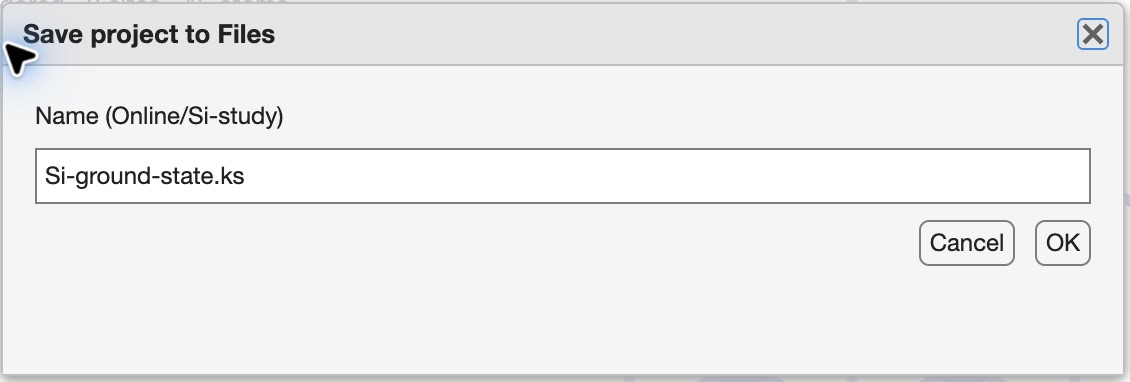
\includegraphics[width=\linewidth]{publication-assets/crop-5eed673aca0b27c69288.png}
\caption{The server-side project save dialog. The filename is Si-ground-state.ks, and the selected \file{Online/Si-study} directory is shown in parentheses.}
\label{fig:online-save-project}
\end{figure}

Enter a filename, not a full server path. The dialog uses the selected directory and appends \file{.ks} if you omit it. Subsequent \ui{Save} operations update this project file.

Once a project has a save location, selecting another folder in Files does not change where Save writes it. Use \ui{Save As...} to rename it, keep a milestone copy, or move to another directory. The Files menu's \ui{Save project to Files} also asks for a name and can save the current project into the selected directory.

\begin{figure}[!htb]
\centering
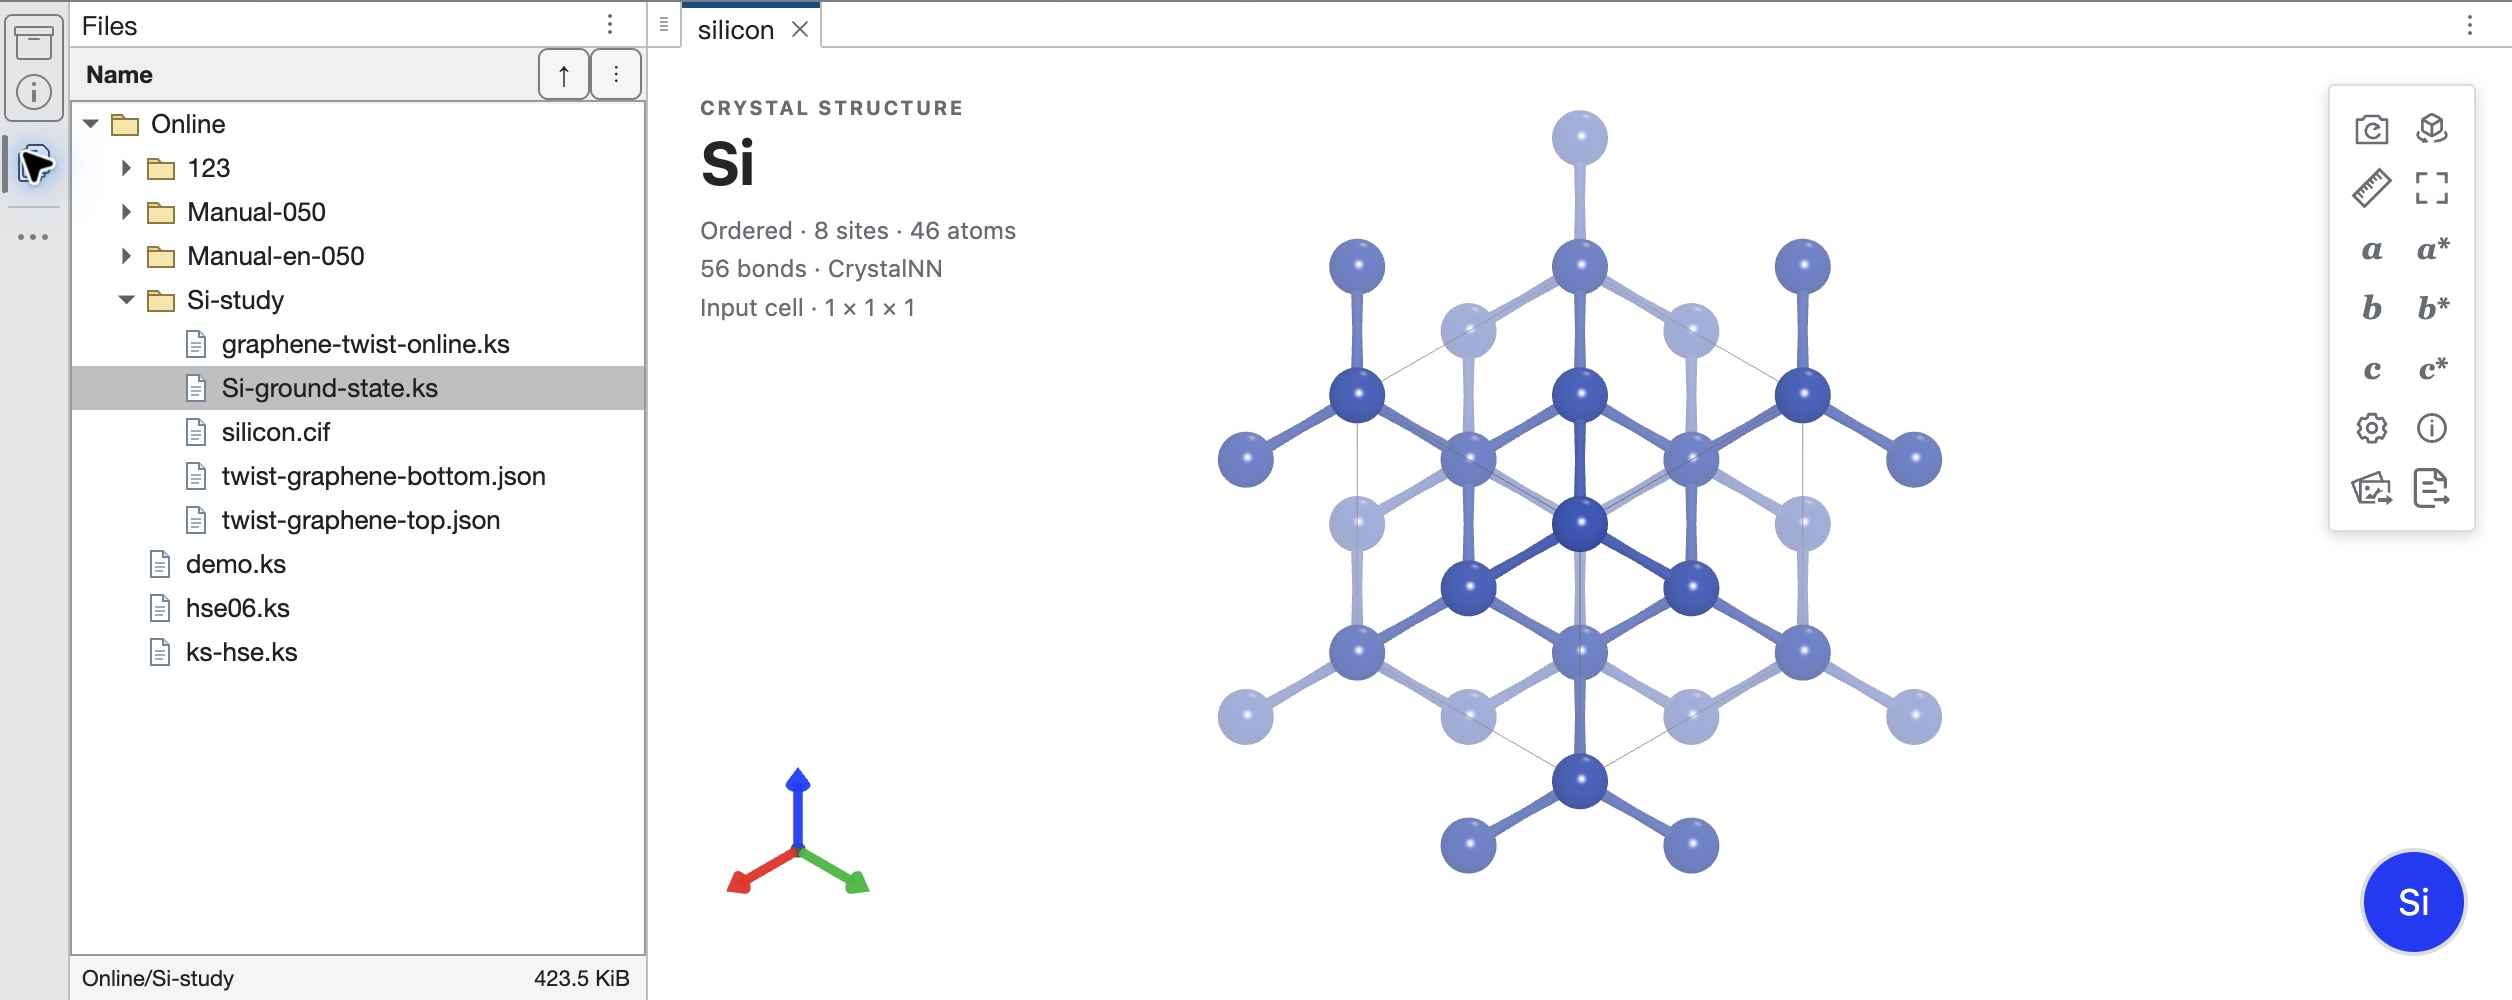
\includegraphics[width=\linewidth]{publication-assets/crop-11fbbbc4e8e9d6f1929d.png}
\caption{The relationship between files and the model. Si-ground-state.ks is selected in Si-study on the left. The central view contains 8 independent sites and 46 displayed atoms including periodic images.}
\label{fig:online-workspace-silicon}
\end{figure}

In Figure~\ref{fig:online-workspace-silicon}, 8 sites is the model's site count; 46 atoms includes periodic images. The project in this section saves the silicon structure. Chapter~\ref{ch:workflows} covers its ground-state calculation.

\subsection{Save a comparison copy}
\index{Save As}

Materials modeling often involves comparing supercells, defects, or parameters. Save a milestone project before a major change to make those comparisons easier to follow. Here, practice Save As without changing the model.

\begin{steps}
\item Select the destination directory in \ui{Files}.
\item Open the save menu and choose \ui{Save As...}.
\item Enter a new name, such as \file{Si-comparison.ks}.
\item Check that the new file appears and the original remains.
\end{steps}

After Save As, further edits apply to the new project file. Names can identify the material, operation, and stage, such as a silicon primitive cell, silicon supercell, or optimized geometry. You need not pack every calculation parameter into a filename; the project retains the detailed settings.

\section{Bring a project back to your computer}
\index{Downloading projects}

\subsection{Download a server-side file}

Server-side saving lets you resume work after signing in again. Local downloads provide backups or copies for sharing. Use both where appropriate. A download contains the file's currently saved contents, so save before downloading.

\begin{steps}
\item Select \file{Si-ground-state.ks} or your comparison project.
\item Choose \ui{Download} from the context menu or \ui{⋮}.
\item Wait for file preparation. Chrome may open a local save dialog immediately; choose a folder, check the project name, and click \ui{Save}.
\item If no system dialog opens, use the in-page \ui{Save as…} action or \mbox{\ui{Browser download}} to use the browser's native download mechanism.
\item Wait for the browser's download list to report completion. If the transfer window has a \ui{Finish} button, click it only after confirming that the local file was saved.
\item Check the project filename and size in your local file manager.
\end{steps}

\begin{figure}[H]
\centering
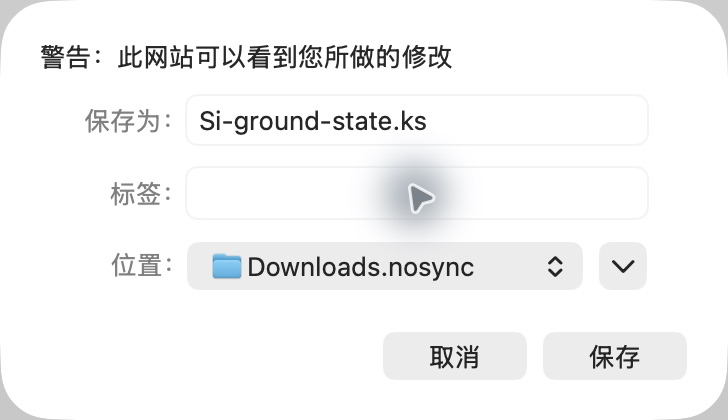
\includegraphics[width=72mm]{publication-assets/crop-348b0d07fb6f4cdab9d3.png}
\caption{The local macOS save dialog for the supplied silicon project. Choose a directory, check the project name, and save. The browser may add a number if a file with the same name exists. System dialog labels follow the operating system language.}
\label{fig:online-project-download}
\end{figure}

Your browser may save directly into Downloads or ask for a location each time. Check its download list if you are unsure where a file went. \ui{Ready to download} in an in-page dialog means that preparation is complete, but you must still finish local saving through \ui{Save as…}, \mbox{\ui{Browser download}}, or the download link. The preparation dialog may close after local saving. Confirm success from the browser's completion status and the actual local file.

If preparation fails, the window may offer \ui{Retry download}; use it to prepare the file again. Canceling a download does not undo a completed server-side save. Select the same file later to try again.

\subsection{Transfer limits}

An individual upload or download can be at most 128~MiB. One upload batch can contain at most 100 files totaling no more than 128~MiB. These are browser transfer limits, not the account's total storage allocation.

Projects can grow substantially as calculation results accumulate. Check the size in Files before downloading. For files above the transfer limit, use the large-file transfer mechanism provided by your deployment.

The structure project saved and downloaded here is supplied as \file{examples/Si-ground-state.ks}. Use it to check the silicon structure and practice the Online file round trip.

\section{Check the current account}

An Online workspace connected to the account service displays the account name at the top. Open its menu and choose My Account to view the account settings page, or open that page through \ui{Home → Settings}. It shows the account name, connection status, and the inactivity limit set by the deployment.

\begin{steps}
\item Check that the displayed name is your account, then open My Account.
\item Check the connection status. A green dot and connected message identify the current session. The inactivity limit is how long a session is kept without interaction.
\item If the connection needs restoring, use \ui{Reconnect}, then check the project and Files after returning to the workspace.
\item Save your project before finishing. Use \ui{Sign out} when you want to leave the account.
\end{steps}

If your deployment does not provide an account settings page, connect through its entry page.

\section{Leave the workspace}

\subsection{Return to the entry page temporarily}

The account menu's exit action returns to the entry page while retaining the workspace until its inactivity limit. With the current browser tab retained, the portal's reconnect action returns to the original interface. This is useful for checking the portal before continuing your work.

Returning to the portal is different from signing out. It does not immediately release computing resources or automatically save the project to disk. Save important changes first.

After completing the hydrogen calculation in Chapter~\ref{ch:first}, practice returning and reconnecting with its saved project:
\begin{steps}
\item Save the current project and check that the calculation has finished.
\item Open the account menu and choose the action to exit KSSOLV Toolbox. Read the workspace-retention notice and confirm to return to the portal.
\item Check that the portal reports that the workspace is still running, then reconnect.
\item In the restored workspace, check the original project. Its SCF workflow should still contain Configuration, SCF, and Plot nodes; Results should retain the Run SCF dataset and EnergyConvergence plot. Open the plot to continue inspecting it.
\end{steps}

\begin{figure}[!htb]
\centering
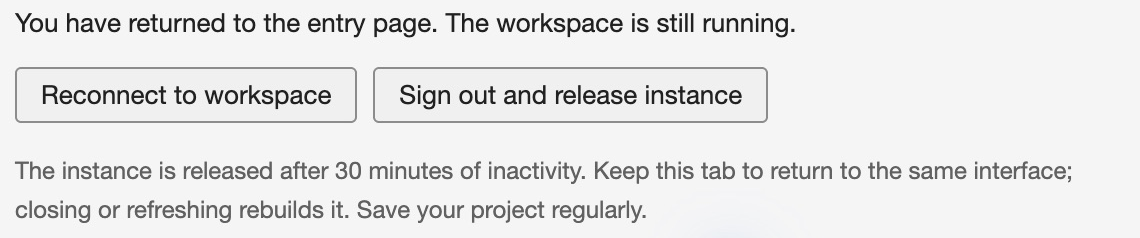
\includegraphics[width=122mm]{publication-assets/crop-432edbee8ecb03b7c537.png}
\caption{Workspace status and the reconnect action after returning to the portal. Reconnect returns to the original project; signing out and releasing the instance ends the workspace.}
\label{fig:online-reconnect}
\end{figure}

\subsection{Close or refresh the page}
\index{Reconnecting}

Closing the page does not sign you out. Return to the same service entry page while the original workspace is still alive to reconnect and rebuild the browser interface. Projects, open structures, and workflows can be restored within that running instance, but temporary dialogs, undo history, and the complete layout are not guaranteed to remain unchanged.

Refreshing rebuilds the browser interface. After a brief network interruption, wait for recovery or reconnect through the service entry page. For a temporary departure, return to the portal through the account menu and reconnect when ready.

\subsection{Sign out and release the workspace}

When you finish, particularly on a shared computer, save the project and use \ui{Sign out} in the account menu, or the portal's sign-out-and-release action. Confirmation ends the access session and releases the running instance.

Your next sign-in uses the same account's saved files and settings. In-memory variables, unsaved edits, and running calculations cannot be relied on to survive sign-out. Save before leaving and download a file if you need a local copy.

\subsection{Understand inactivity release}

The platform sets the inactivity limit. Check account settings or portal notices for the current value. Deployments may use different limits, and a warning appears as release approaches. Keyboard, mouse, touch, and scroll interactions count as activity. Merely leaving the tab in the foreground or allowing status updates does not extend the limit.

A running calculation does not itself imply user interaction. Before scheduling a long task, check your platform's policy for inactivity release and long calculations. Follow your cluster's instructions for independent batch queues. Chapter~\ref{ch:remote} covers remote submission from the full MATLAB\regmark{} toolbox.

\Needspace{6\baselineskip}
\begin{notebox}{Resume after signing in again}
Find the exercise directory in Files and double-click the saved \file{.ks} project to continue editing structures, configuring workflows, or viewing results.
\end{notebox}

\section{Manage the workspace connection}

The resource status at the bottom shows CPU and memory usage for the current environment. In deployments allocating resources per account, it describes the current workspace's allocation. A plain container deployment may instead show the host environment. Use the status labels and deployment documentation to identify the scope of the reported resources.

Workflow resource options depend on the node's task, solver method, and deployment capabilities. Select a node and inspect its resource panel; Section~\ref{sec:node-resources} explains the choices and checks. The Home tab's \ui{Parallel} button does not replace node resource settings. Process-pool and GPU availability must also be checked against the server environment.

Once comfortable with files, continue with the hydrogen calculation in Chapter~\ref{ch:first}. Upload the supplied \file{h2.cif} into your server-side directory and import it into the project. Create the SCF workflow and enter that chapter's structure and solver settings.

Figure~\ref{fig:online-h2-config} shows the hydrogen tutorial's structure input. Select the node, choose \ui{Workflow → Configure Node}, and scroll to \ui{Options}. The node labeled \ui{Configuration} performs the \ui{Build Molecule} task. Choose Molecule, structure h2, PBE, default pseudopotentials, 20 Ha, 0 K, and Nspin=1. Set the SCF method and iteration limit as in Chapter~\ref{ch:first}.

\begin{figure}[!htb]
\centering
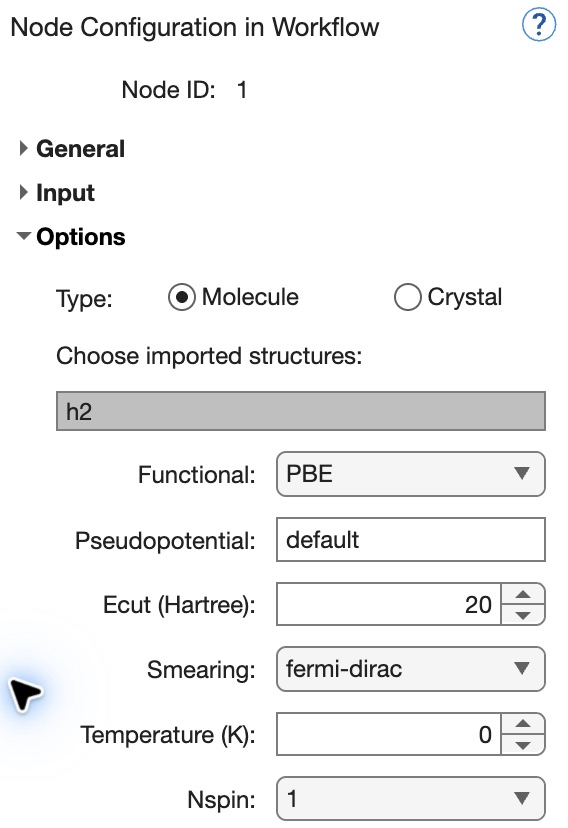
\includegraphics[width=88mm]{publication-assets/crop-434fe0ac4d3f46cfaf46.png}
\caption{Structure-input options for the hydrogen workflow. Check the selected h2 structure and calculation settings in the Config Editor on the right.}
\label{fig:online-h2-config}
\end{figure}

The reference calculation converges in 7 iterations; Chapter~\ref{ch:first} gives the log and numerical results. After completion, open the Project Browser and expand \ui{Results}. \ui{Run SCF} under \ui{Datasets} holds the run data; \ui{EnergyConvergence} under \ui{Plots} opens the convergence plot.

After checking the log and curve, save again, close the project, and double-click its saved \file{.ks} file in \ui{Files} to reopen it. Figure~\ref{fig:online-h2-results} shows the reopened project's result groups, with datasets and plots stored separately. Double-click \ui{EnergyConvergence} again to inspect the seven-iteration history. Finally, download the project for a local copy.

\begin{figure}[!htb]
\centering
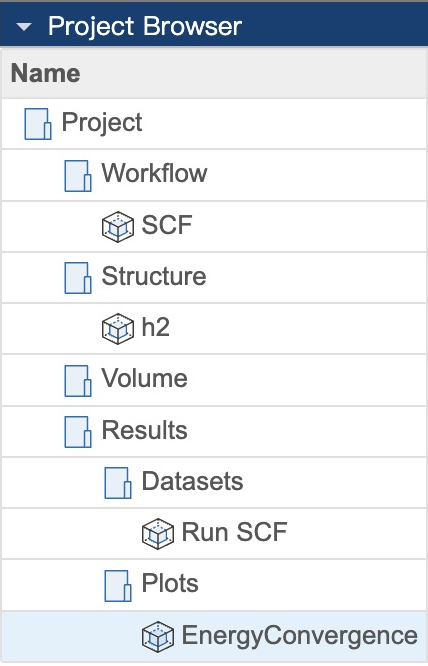
\includegraphics[width=55mm]{publication-assets/crop-c36a9eee3be02622a4d7.png}
\caption{Results in the hydrogen project. Results contains the Run SCF dataset and EnergyConvergence plot. Double-click the plot entry to view the iteration history.}
\label{fig:online-h2-results}
\end{figure}

This completes the sequence from structure preparation through server-side calculation, saving, and reopening.

If connection fails, return to the entry page and check whether the workspace is still starting. Use its retry action first when offered. For a persistent problem, the portal may provide a restart action. Restarting retains saved files and settings but ends the in-memory session; confirm that this is appropriate before proceeding.

If you forget your password, use the recovery action on the sign-in page to retrieve your recovery question, then enter the answer and a new password. Resetting ends existing sessions. Sign in again after success. Contact the administrator if no question was set or you cannot remember the answer.

If the interface reports \ui{Persistent Files is unavailable in this deployment.}, upload local files to open them and download through the browser when saving. Confirm that you have a local copy before leaving.
